\graphicspath{{members/tf/figures/}}

\subsection{Pipeline A (sollte schon bei Saman anfgangen)}
\input{members/tf/authors}
\subsubsection{Area transition}
In previous steps we used clustering to estimate the fraction of pixels in the image from above that display leave surface. But this value is only a fraction and no area measure jet.\\
To translate that fraction into an area we have to find the total area that the camera observes first. To do that we take a look at the camera setup again. \ref{fig:setupAbove}
   \begin{figure}[H]
       \centering
       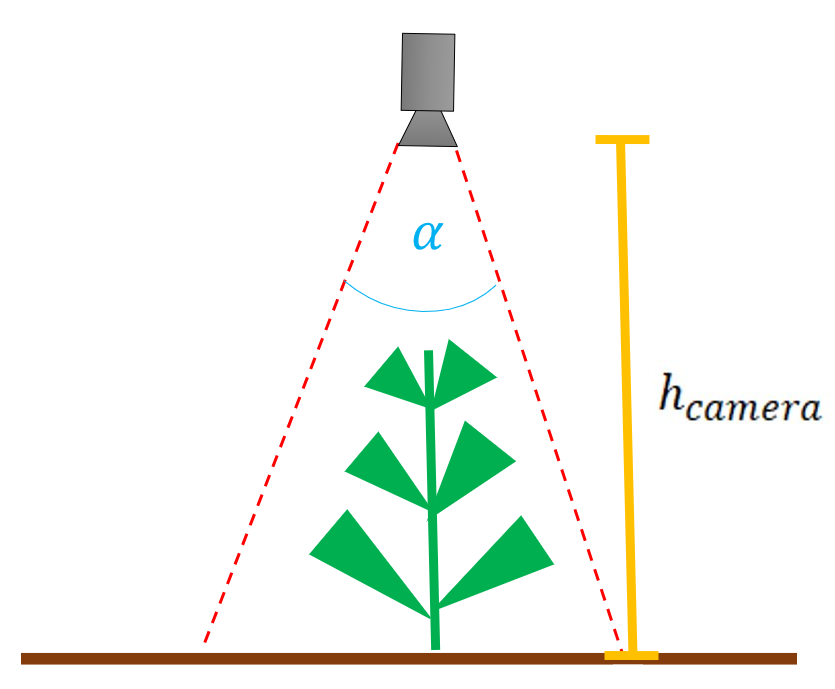
\includegraphics[scale=0.6]{setupAbove.PNG}
       \caption{Setup of the camera above the plant. $\alpha$ denotes the lense angle in which the camera captures the picture. $\alpha$ and $h_{Camera}$ are known.}
       \label{fig:setupAbove}
   \end{figure}
By only looking at half of the cone that the camera covers we can spot a triangle with a $90^{\circ}$ angle. Furthermore the height of the trianlge is $h_{Camera}$, the angle in the upper corner is $\frac{\alpha}{2}$ and the bottom side has a length of half the width of the observed area. The width of the observed area, calculated from the triangle needs to be squared, to get the area of the squared image:\\
$$A_{Camera} = (2\cdot h_{Camera}\cdot tan(\frac{\alpha}{2}))^2$$
$A_{Camera}$ only needs to be calculated once, as long as the camera parameters don't change. To calculate the area of the observed green, we simply multiply the captured area of the camera with the fraction $p_{Green}$ calculated by the clustering: 
$$A_{Observed} = p_{green}\cdot A_{Camera}$$
\textbf{Note:} This whole process works as long as the camera is set as supposed. A tilted camera would break the results since the used triangle would no longer have a $90^{\circ}$ angle. A tilted camera might also unintentionally capture adjacent plants.\\
\textbf{Model:} The observed plants are relatively small (max 40cm) in relation to the height of the camera (min 2m). Hence the plants can be considered to be flat on the ground, without changing the visible area. This assumption breaks when the plants grow much larger than expected. However this is pretty uncommon and can be therfore be neglected.
\subsubsection{Tilt angle correction}
The area calculated in the previous section represents the green area seen from above, which is not the area of the leaves in the canopy we are searching for. That's because the leaves aren't aligned horizontal but tilted and therefore their size is not perfectly captured as seen in \ref{fig:tiltedLeaf}. We have to add a correction to the obseved area to estimate the canopy area.\\
   \begin{figure}[H]
       \centering
       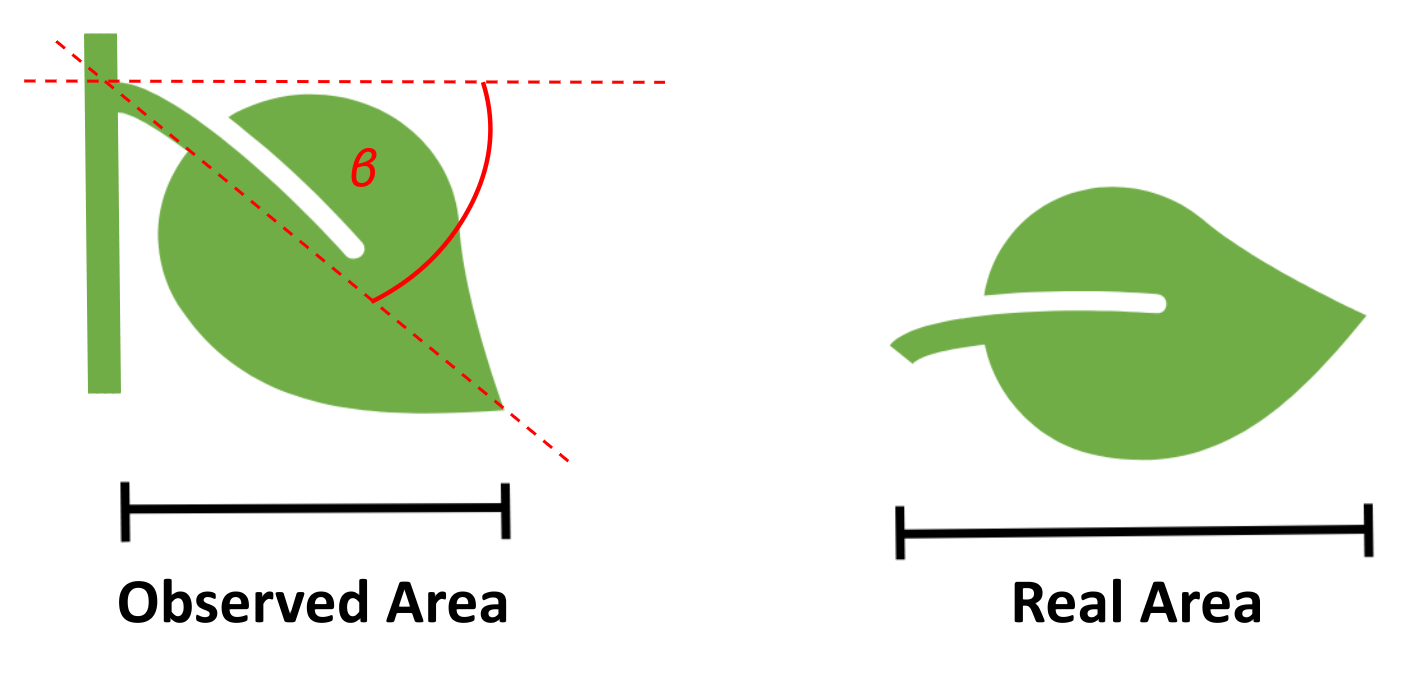
\includegraphics[scale=0.6]{tiltedLeaf.PNG}
       \caption{Sideview comparision of an untilted and a tilted leaf. The captured area from above reduces as a leaf gets tilted by an angle $\beta$.}
       \label{fig:tiltedLeaf}
   \end{figure}
The single leaves are assumed to be uncurved planes, therefore the observed area, the real area and the tilt angle $\beta$ form a $90^{\circ}$ triangle in the 2D sideview. Hence:
$$A_{Canopy} \approx \frac{A_{Observed}}{\arccos \langle |\beta |\rangle }$$
the absolute value of $\beta$ is used in this formula, because wether the tilting is upwards and downwards does not effect the visible area. furthermore the mean of $\beta$ is used, since the single tilt angles of the leaves are unknown and hard to estimate. That mean denotes the mean over all plants, not just a single one. However $\langle |\beta |\rangle$ is still hard to estimate, therefore $\arccos \langle |\beta |\rangle$ is replaced by a parameter that will be trained once the model is in use.\\
\textbf{Model: } The leaves are modeled as uncurved planes, which is most likely not true. Nevertheless the transform described in this section is expected to work, because the trained factor is will not only be trained to correct tiltangles but also curvature of the leaves. Using the model will show whether a linear model can learn this transformation. Assuming that each leaf is scaled by a factor, a linear model should do just fine. Coverage of leaves, which might also occure with adjacent leaves and affect the observed area will be discussed in section \ref{section:EstLAI}.
\subsection{Pipeline B}
\input{members/tf/authors}
The Area of the canopy, that was calculated in the revious section only tells us about the width of the plant but not the total leaf area. The area alone can not divide the difference between a tall relatively thin plant and a small relatively wide plant as they might have the same canopy green area but a different Leaf Area Index. The same is for a tall plant that is not thin but has large brown areas making the measured canopy small just like a thin plant.\\
Therefore the height gets measured aswell, to capture the size of the plant better. The Pipeline in \ref{fig:pipelineB} shows, how a picture from the side is used to determite the top of the plant. First of all an edge detector is applied on the picture. Then the longest edge (the pole behind the plant) is found. To find the top of the plant a small window slides down the post until it detects green covering the pole. That point will be considered as the top of the plant. From that point and the camera setup the hieght can be calculated. 
   \begin{figure}[H]
       \centering
       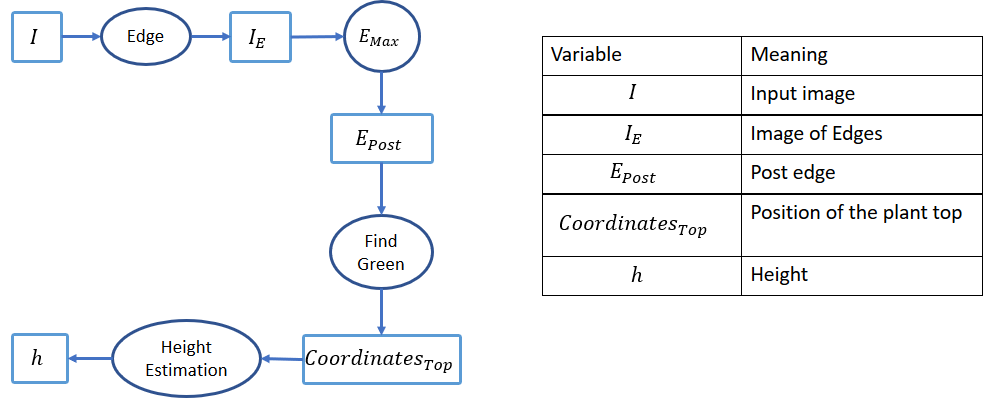
\includegraphics[scale=0.6]{pipelineB.PNG}
       \caption{Pipeline to estimate the height of the plant.}
       \label{fig:pipelineB}
   \end{figure}
\subsubsection{Height estimation setup}
The camera  is set as seen in \ref{fig:setupSide}. The camera is set at a certain height ($h_camera$), a certain distance from the plant ($d$) and has a known tilt angle $\alpha$. The camera slides over a rail, that has a constant distance to the plantlanes and a constant height, to make sure the setup stays the same for every plant.
   \begin{figure}[H]
       \centering
       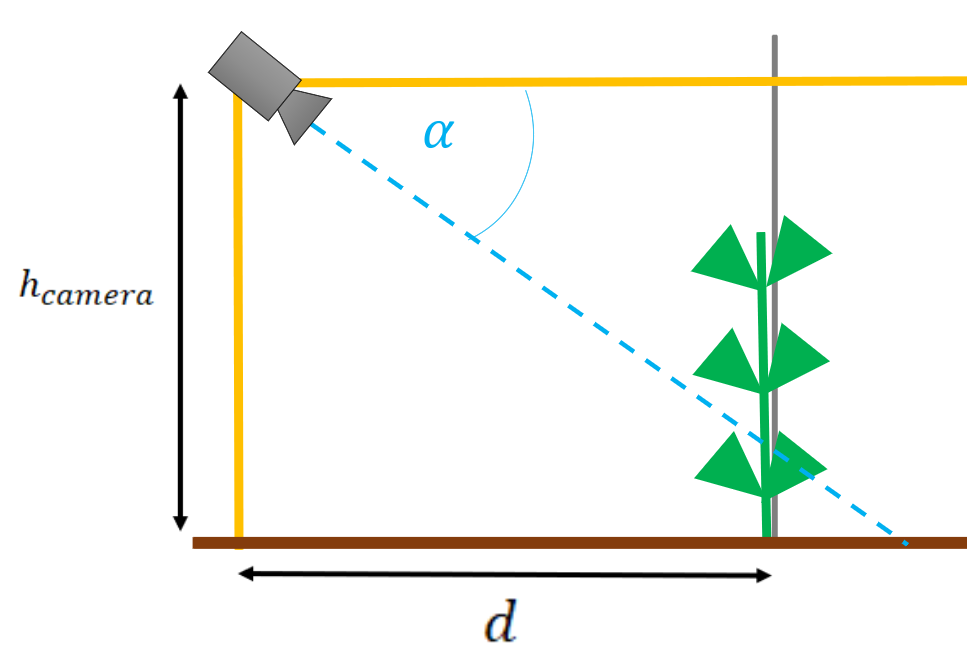
\includegraphics[scale=0.6]{setupSide.PNG}
       \caption{Setup of the camera on the side of the plant. $\alpha$ denotes the tilt angle of the camera as its slightly facing down. }
       \label{fig:setupSide}
   \end{figure}
Furthermore every plant has a pole that is placed behind the plant from the cameras perspective, this helps the plant grow straight one one hand but is also usefull for the procedure described below. it is important that the pole is large enough to exit the top of the camera frame and is as straight as possible.
\subsubsection{Estimating top of plant}
To estimate the top of the plant the pole must be found first. that is done using edge detection.
\subsubsection{Edge detection}
to detect the edges a simple kernel was applied to the whole picture.\\
TODO:\\
-create pictures with Edges (display kernel)\\
-sum all coumns up\\
-find biggest edge (maybe another kernel)\\
-align window (start at top, go down)\\
Once biggest vertical edge is found, a little window of $10\times10$ (larger?/smaller?) pixels is layed on the top of the pole, this is done bay putting it on the top of the picture and the position where the biggest edge was found. This might not directly hit the pole, since it might be tilted. To be invariant to little tiltings in the pole, a correction is applied. If the window covers mostly grey pixels (pole), the pole is found. A threshold for the amount of of grey pixels needed for the window to be considered mostly grey should be tested once the system is implemented. If the window does not cover mostly grey the areas left and right of the window are searched for grey areas that fulfill the threshold. In detail the window is shifted left and right of the original position until a position is found where the threshold is fulfilled. The search for the top of the pole should be limited by a certain distance from the biggest edge to prevent other poles from plants in the background to be found.\\
Once the top of the pole is found, the window starts moving down the pole pixel by pixel. After every step the window is tested to fulfill the threshold, if it does, the search continues with the next step. If the threshold is not fulfilled the window does no longer cover the pole, either because the pole is covered by leaves at that height or because the pole is tilted and the window lost track of it by moving straight down. To prevent the window from losing track of the pole while its still uncovered the same correction is apllied that was already used to find the top of the plant, the window searches sideways If it doesn't find a grey area on the left or the right it is because the pole is covered by leaves. Hence the top of the plant is found when the correction can't find a grey area near the old position.\\ 
Once the top of the plant is found by the described procedure the coordinates of the pixel where the search lost track of the pole are stored.
\textbf{Invariances:} The approach with the pole was choosen, to be invariant to green in the background of the picture. That way the plants can be planted close to each other without any problem for this procedure, because no other plant will cover the focused plants pole.\\
The procedure is invariant to slighly tilted poles, since the window is correcting its path every step, but if the pole is tilted to much the top of the pole might not be found. A strongly tilted pole might also affect the results in a negative way since the pole could be entering the plant surface rather from the side than from the top, which would be lower than the top actually is.

\subsubsection{Height estimation}
Once the top of the plant is found in the image, its coordinates need to be translated into the actual height of that plant. To do so we take advantage of our knowledge about the camera setup displayed in \ref{fig:estHeight}.
   \begin{figure}[H]
       \centering
       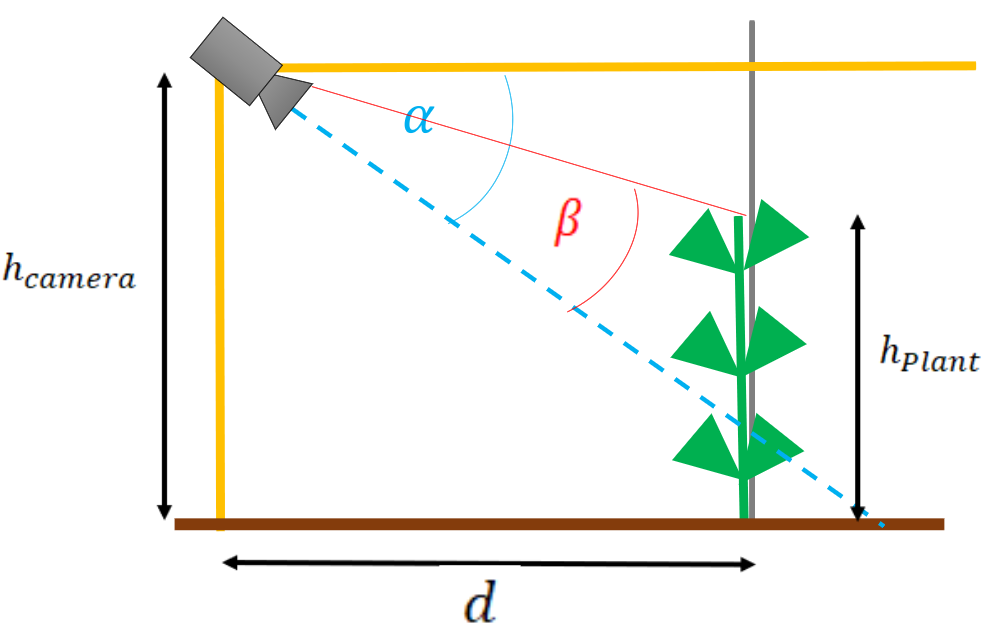
\includegraphics[scale=0.6]{estHeight.PNG}
       \caption{Setup of the camera on the side of the plant. $\alpha$ denotes the tilt angle of the camera as its slightly facing down. $\beta$ denotes the vertical angle between the center of the picture and the top of the plant. }
       \label{fig:estHeight}
   \end{figure}
Once we know the angle $\beta$ we can easily calculate the height of the plant, since we have a $90^{\circ}$ triangle in our setup. The angle $\beta$ is calculated as follows, where $\gamma$ denotes the lens angle, which states the maximum angle the camera captures:\\
   \begin{figure}[H]
       \centering
       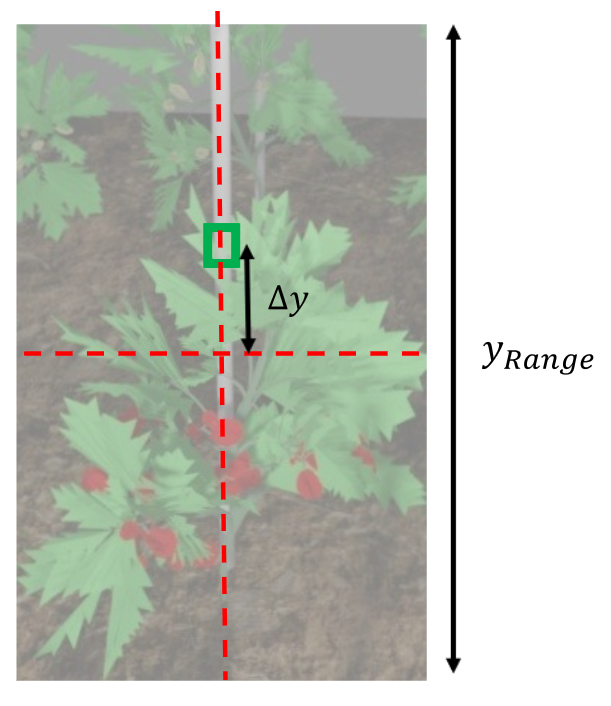
\includegraphics[scale=0.6]{getTopAngle.PNG}
       \caption{$\Delta y$ denotes the vertical distance between the center and the top of the plant in pixels (can be negative if the top is below the center). $y_{range}$ denotes the vertical resolution of the picture.}
       \label{fig:getTopAngle}
   \end{figure}
$$\beta = \frac{\Delta y}{(\frac{y_{range}}{2})}\gamma$$
\textbf{Note:} This works well as long as the picture is not distorted by the lens. Thus its suggested not to use a wide angle lens, since those distort the image unlike regular lenses.\\
Once we know $\beta$ we can calculate the height of the plant :
$$h_{plant} = h_{camera} - d\cdot tan(\alpha - \beta)$$
\textbf{Model:} The plant is modeled as a cylinder in this step. Hence it is assumed that the first point of the pole that is covered is actually the top. That this idea works quite well is shown in \textcolor{red}{ABSCHNITT IMPLEMENTATION. (STIMMT DAS ?)}
\subsection{Estimating LAI}
\label{section:EstLAI}

Beachte Überdeckungen innerhalb einer Ebene
\subsection{Yield prediction}
%Lorem ipsum dolor sit amet, consetetur sadipscing elitr, sed diam nonumy eirmod tempor invidunt ut labore et dolore magna aliquyam erat, sed diam voluptua. At vero eos et accusam et justo duo dolores et ea rebum. Stet clita kasd gubergren, no sea takimata sanctus est Lorem ipsum dolor sit amet. Lorem ipsum dolor sit amet, consetetur sadipscing elitr, sed diam nonumy eirmod tempor invidunt ut labore et dolore magna aliquyam erat, sed diam voluptua. At vero eos et accusam et justo duo dolores et ea rebum. Stet clita kasd gubergren, no sea takimata sanctus est Lorem ipsum dolor sit amet. Lorem ipsum dolor sit amet, consetetur sadipscing elitr, sed diam nonumy eirmod tempor invidunt ut labore et dolore magna aliquyam erat, sed diam voluptua. At vero eos et accusam et justo duo dolores et ea rebum. Stet clita kasd gubergren, no sea takimata sanctus est Lorem ipsum dolor sit amet.

Duis autem vel eum iriure dolor in hendrerit in vulputate velit esse molestie consequat, vel illum dolore eu feugiat nulla facilisis at vero eros et accumsan et iusto odio dignissim qui blandit praesent luptatum zzril delenit augue duis dolore te feugait nulla facilisi. Lorem ipsum dolor sit amet, consectetuer adipiscing elit, sed diam nonummy nibh euismod tincidunt ut laoreet dolore magna aliquam erat volutpat.
